
\lecture{Confidence Intervals Part II}{confidence-interval-II}
\section{Confidence Intervals Part II}

\title{Confidence Intervals}
\subtitle{Part II - Putting them to Use}

\author{Kelly Black}
\institute{Clarkson University}
\date{2 March 2012}

\begin{frame}
  \titlepage
\end{frame}

\begin{frame}
  \frametitle{Outline}
  \tableofcontents[pausesection,hideothersubsections,sectionstyle=show/hide]
\end{frame}


\subsection{Clicker Quiz}


\begin{frame}
  \frametitle{Clicker Quiz}

  You run an experiment multiple times. Each time you generate data
  and calculate a sample mean. The sample means are plotted below with
  circles, and the true mean is the square. The estimator appears to
  be \rule{3cm}{.2mm} .

  \vfill

  \centerline{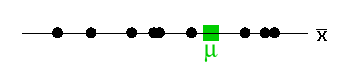
\includegraphics[width=5cm]{img/negativeBias}}

  \vfill

  \begin{tabular}{l@{\hspace{3em}}l@{\hspace{3em}}l@{\hspace{3em}}l}
    A: Negatively Biased  & B: Unbiased  & C: Positively Biased
  \end{tabular}

  \vfill
  \vfill
  \vfill

\end{frame}


\subsection{Confidence Intervals}


\begin{frame}

  \centerline{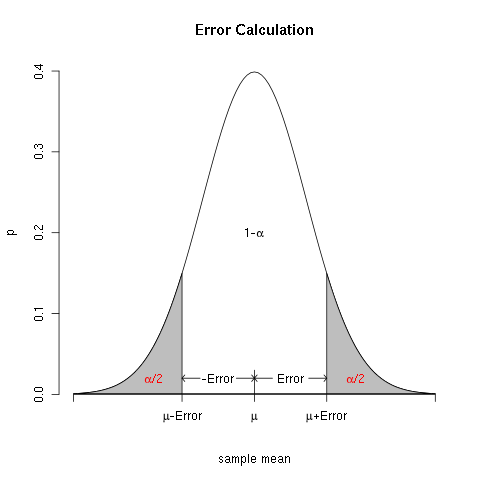
\includegraphics[width=6cm]{img/confidenceInterval}}

  \begin{block}{The Error Relationship for Confidence Intervals}
    \begin{eqnarray*}
      p\lp z \leq \frac{-error}{\frac{\sigma}{\sqrt{n}}}\rp & = & \frac{\alpha}{2}.
    \end{eqnarray*}
  \end{block}

\end{frame}


\begin{frame}{The Confidence Interval}
  \begin{definition}
    The \textit{confidence interval} is an interval that likely
    includes the true mean.
  \end{definition}
\end{frame}

\subsection{Examples}


\begin{frame}
  \frametitle{Example}

  We call up and ask twenty factory operators in a given sector what
  their yearly output is in dollars. The sample mean is \$450,000 and
  the standard deviation is \$50,000. Find the 95\% confidence
  interval.

  \vfill

  \only<2->{
    \textit{
      The 95\% confidence interval is from \$471,913 and \$428,087
      assuming a normal distribution with twenty samples.
    }
  }

  \vfill

\end{frame}


\begin{frame}
  \frametitle{Example}

  You read a report that says that eighteen companies in a given
  sector were polled, and the confidence interval for the yearly
  output in dollars is between \$710,000 and \$650,000 with a standard
  deviation of \$96,000. What is the significance level?

  \vfill

  \only<2->{
    \textit{
      There is a probability of about 18\% that the true mean is not
      between \$710,000 and \$650,000.
    }
  }

  \vfill

\end{frame}


\begin{frame}
  \frametitle{Example}

  You are asked to determine a 95\% confidence interval for the mean
  yearly output in dollars for the companies in a given sector. You
  are told that the error should be about \$30,000. From the reports
  that you have read it looks like the standard deviation is about
  \$100,000. How many companies should you poll?

  \vfill

  \only<2->{
    \textit{
      Assuming a normal distribution you will need to poll at least 43
      companies to get a 95\% confidence interval with an error of \$30,000.
    }
  }

  \vfill


\end{frame}



% LocalWords:  Clarkson pausesection hideallsubsections
